% !TEX TS-program = XeLaTeX
% use the following command:
% all document files must be coded in UTF-8
\documentclass[spanish]{textolivre}
% build HTML with: make4ht -e build.lua -c textolivre.cfg -x -u article "fn-in,svg,pic-align"

\journalname{Texto Livre}
\thevolume{16}
%\thenumber{1} % old template
\theyear{2023}
\receiveddate{\DTMdisplaydate{2022}{12}{7}{-1}} % YYYY MM DD
\accepteddate{\DTMdisplaydate{2022}{12}{15}{-1}}
\publisheddate{\DTMdisplaydate{2023}{1}{3}{-1}}
\corrauthor{Manuel Francisco Romero Oliva}
\articledoi{10.1590/1983-3652.2023.42047}
%\articleid{NNNN} % if the article ID is not the last 5 numbers of its DOI, provide it using \articleid{} commmand 
% list of available sesscions in the journal: articles, dossier, reports, essays, reviews, interviews, editorial
\articlesessionname{dossier}
\runningauthor{Romero Oliva et al.} 
%\editorname{Leonardo Araújo} % old template
\sectioneditorname{Daniervelin Pereira}
\layouteditorname{Thaís Coutinho}

\title{Promoción de la lectura y transmedia. De la creación editorial al book-trailer como epitexto ficcional}
\othertitle{Promoção da leitura e transmídia. Da criação editorial ao book trailer como um epitexto fictício}
\othertitle{Reading promotion and transmedia. From editorial creation to the book-trailer as a fictional expitext}
% if there is a third language title, add here:
%\othertitle{Artikelvorlage zur Einreichung beim Texto Livre Journal}

\author[1]{Manuel Francisco Romero Oliva~\orcid{0000-0002-6854-0682}\thanks{Email: \href{mailto:manuelfrancisco.romero@uca.es}{manuelfrancisco.romero@uca.es}}}
\author[1]{Hugo Heredia Ponce~\orcid{0000-0003-3657-1369}\thanks{Email: \href{mailto:hugo.heredia@uca.es}{hugo.heredia@uca.es}}}
\author[1]{Carmen Romero Claudio~\orcid{0000-0002-2813-9579}\thanks{Email: \href{mailto:carmen.romeroclaudio@gmail.com}{carmen.romeroclaudio@gmail.com}}}
\affil[1]{Universidad de Cádiz, Facultad de Ciencias de la Educación, Departamento de Didáctica de la Lengua y la Literatura, Cádiz, España.}

\addbibresource{article.bib}
% use biber instead of bibtex
% $ biber article

% used to create dummy text for the template file
\definecolor{dark-gray}{gray}{0.35} % color used to display dummy texts
\usepackage{lipsum}
\SetLipsumParListSurrounders{\colorlet{oldcolor}{.}\color{dark-gray}}{\color{oldcolor}}

% used here only to provide the XeLaTeX and BibTeX logos
\usepackage{hologo}

% if you use multirows in a table, include the multirow package
\usepackage{multirow}

% provides sidewaysfigure environment
\usepackage{rotating}

% CUSTOM EPIGRAPH - BEGIN 
%%% https://tex.stackexchange.com/questions/193178/specific-epigraph-style
\usepackage{epigraph}
\renewcommand\textflush{flushright}
\makeatletter
\newlength\epitextskip
\pretocmd{\@epitext}{\em}{}{}
\apptocmd{\@epitext}{\em}{}{}
\patchcmd{\epigraph}{\@epitext{#1}\\}{\@epitext{#1}\\[\epitextskip]}{}{}
\makeatother
\setlength\epigraphrule{0pt}
\setlength\epitextskip{0.5ex}
\setlength\epigraphwidth{.7\textwidth}
% CUSTOM EPIGRAPH - END

% LANGUAGE - BEGIN
% ARABIC
% for languages that use special fonts, you must provide the typeface that will be used
% \setotherlanguage{arabic}
% \newfontfamily\arabicfont[Script=Arabic]{Amiri}
% \newfontfamily\arabicfontsf[Script=Arabic]{Amiri}
% \newfontfamily\arabicfonttt[Script=Arabic]{Amiri}
%
% in the article, to add arabic text use: \textlang{arabic}{ ... }
%
% RUSSIAN
% for russian text we also need to define fonts with support for Cyrillic script
% \usepackage{fontspec}
% \setotherlanguage{russian}
% \newfontfamily\cyrillicfont{Times New Roman}
% \newfontfamily\cyrillicfontsf{Times New Roman}[Script=Cyrillic]
% \newfontfamily\cyrillicfonttt{Times New Roman}[Script=Cyrillic]
%
% in the text use \begin{russian} ... \end{russian}
% LANGUAGE - END

% EMOJIS - BEGIN
% to use emoticons in your manuscript
% https://stackoverflow.com/questions/190145/how-to-insert-emoticons-in-latex/57076064
% using font Symbola, which has full support
% the font may be downloaded at:
% https://dn-works.com/ufas/
% add to preamble:
% \newfontfamily\Symbola{Symbola}
% in the text use:
% {\Symbola }
% EMOJIS - END

% LABEL REFERENCE TO DESCRIPTIVE LIST - BEGIN
% reference itens in a descriptive list using their labels instead of numbers
% insert the code below in the preambule:
%\makeatletter
%\let\orgdescriptionlabel\descriptionlabel
%\renewcommand*{\descriptionlabel}[1]{%
%  \let\orglabel\label
%  \let\label\@gobble
%  \phantomsection
%  \edef\@currentlabel{#1\unskip}%
%  \let\label\orglabel
%  \orgdescriptionlabel{#1}%
%}
%\makeatother
%
% in your document, use as illustraded here:
%\begin{description}
%  \item[first\label{itm1}] this is only an example;
%  % ...  add more items
%\end{description}
% LABEL REFERENCE TO DESCRIPTIVE LIST - END


% add line numbers for submission
%\usepackage{lineno}
%\linenumbers

\usepackage{siunitx}
\sisetup{locale = FR}

\begin{document}
\maketitle

\begin{polyabstract}
\begin{abstract}
Este trabajo\footnote{Este trabajo está vinculado a las líneas del proyecto I+D+i PID2021-126392OB-100 “Lecturas no ficcionales para la integración de ciudadanas y ciudadanos críticos en el nuevo ecosistema cultural” –LENFICEC–” y la tesis doctoral Creación de un tercer espacio educativo en la formación inicial para el desarrollo de la competencia informacional y mediática. Un estudio de caso desde los libros ilustrados de no ficción, Programa de doctorado: 8219 Investigación y práctica educativa, Universidad de Cádiz.} pretende analizar el perfil de los epitextos virtuales que aparecen en cuatro plataformas editoriales de ámbito educativo para la promoción del libro. Siendo conscientes de que estamos inmersos en una sociedad gaseosa \cite{scolari2021}% (SCOLARI, 2021) 
 en donde predomina lo breve, las modas y lo viral; el nuevo paradigma de la lectura se corresponde con una hibridación analógico-digital en la que los book-trailer, se convierten en ejemplo claro de producto transmedia del texto original por parte de las editoriales. Nuestra investigación de corte cualitativo se basa en un análisis de corpus de 70 epitextos ficcionales, mediante una lista de contenidos dimensionada en tres categorías de estudio. Los resultados evidencian su presencia tanto en los libros de literatura infantil como juvenil para el fomento de la lectura y generar la curiosidad y el disfrute del prosumidor. Sin embargo, también es necesario resaltar que este tipo de técnicas y lenguajes multimodales no puede suplantar el protagonismo del hecho literario y la lectura en sí misma.

\keywords{Sociedad digital \sep Epitextos editoriales \sep Book-trailer \sep Sector editorial}
\end{abstract}

\begin{portuguese}
\begin{abstract}
Este trabalho tem como objetivo analisar o perfil dos epitexts virtuais que aparecem em quatro plataformas editoriais educacionais para a promoção de livros. Estando conscientes de que estamos imersos em uma sociedade gasosa \cite{scolari2021}%(SCOLARI, 2021) 
onde predominam o breve, a moda e o viral; o novo paradigma de leitura corresponde a uma hibridização analógico-digital na qual os trailers de livros se tornam um claro exemplo de um produto transmídia do texto original pelas editoras. Nossa pesquisa qualitativa se baseia em uma análise de 70 epitexts fictícios, por meio de uma lista de conteúdos dividida em três categorias de estudo. Os resultados mostram sua presença tanto em livros de literatura infanto-juvenil quanto em livros de literatura para adultos jovens, a fim de incentivar a leitura e gerar curiosidade e prazer no prosummer. Entretanto, também é necessário destacar que este tipo de técnicas e linguagens multimodais não podem suplantar o protagonismo do fato literário e da própria leitura.

\keywords{Sociedade digital \sep Epitextos editoriais \sep Book Trailer \sep Setor editorial}
\end{abstract}
\end{portuguese}

\begin{english}
\begin{abstract}
This paper aims to analyse the profile of the virtual epitexts that appear in four educational publishing platforms for the promotion of books. Being aware that we are immersed in a gaseous society \cite{scolari2021} %(SCOLARI, 2021) 
where the brief, fashions and the viral predominate; the new paradigm of reading corresponds to an analogue-digital hybridisation in which book-trailers become a clear example of a transmedia product of the original text by publishers. Our qualitative research is based on a corpus analysis of 70 fictional epitexts, by means of a list of contents divided into three study categories. The results show their presence in both children's and young adult literature books in order to encourage reading and generate curiosity and enjoyment in the prosumer. However, it is also necessary to highlight that this type of multimodal techniques and languages cannot supplant the protagonism of the literary fact and reading itself.

\keywords{Digital society \sep Editorial epitexts \sep Book-trailer \sep Publishing sector}
\end{abstract}
\end{english}
% if there is another abstract, insert it here using the same scheme
\end{polyabstract}

\section{Introducción}\label{sec-intro}
La entrevista realizada por Carlos A. Scolari a Néstor García Canclini \cite{scolari2020cultura} %(SCOLARI, 2020) 
podría ser el punto de partida de nuestro estudio: la cultura digital cambia la lectura y los modos de estudiarla. El canon de lectura se suma a una nueva conceptualización en relación con múltiples receptores y factores condicionantes de sus desarrollos \cite{ezquerro2022comunicacion}, %(MARTÍNEZ ESQUERRO, 2022), 
mediante la hibridación de la cultura letrada y la cultura digital. Pues, como subraya \cite[p.37]{tabernero2022formar}, “el libro, con su fisicidad, dirige y adiestra al lector en esa lectura hipertextual”, propia de la interacción que se genera entre él y la multimodalidad de pantallas \cite{landow2015bueno}. Asistimos a un mundo cambiante y líquido para \textcite{bauman2019}, %Bauman (2019), 
que, en nuestro caso, contemplamos más acertado vincular a la metáfora de \textcite{scolari2021} %Scolari (2021) 
sociedad gaseosa, por su relación con los medios y el consumo; lo viral y la cultura snack en la que nos desenvolvemos: “brevedad, miniaturización, fugacidad, fragmentación, viralidad, remixabilidad, infoxicación, movilidad, aceleración y afterpost.” \cite[p. 157]{scolari2021}. %(SCOLARI, 2021, p.157).
Rasgos en los que la cultura, en general, y la promoción del libro, en particular, se sumergen desde una concepción holística e interdependiente: —\Cref{tbl01}—:

%\setlength\LTleft{-1in}
%\setlength\LTright{-1in}
\begin{small}
\renewcommand{\arraystretch}{1.5}
\begin{longtable}{
    >{\raggedright\arraybackslash}p{0.2\textwidth}
    p{0.72\textwidth}
    }
\caption{Hacia una cultura \emph{snack} en la promoción de la lectura.}
\label{tbl01}
\\
\toprule
\emph{Cultura snack...}\ldots  & \ldots \emph{...en una sociedad gaseosa}\\
\midrule
\emph{Miniaturización y brevedad} & 
La tendencia tecnológica de reducir los dispositivos electrónicos se convierte en una referencia de lo mínimo, que no pasa inadvertida, como epitextos milénicos, en la promoción de la lectura. Un universo de mensajes que viene caracterizado por la “miniaturización” del relato y la brevedad del mensaje en la búsqueda de la interacción en la red. Facebook, Youtube, Whatsapp, Instagram, Twitter, TikTok… conforman una nebulosa de microtextualidades \cite{rodenas2009microtextualidad} en las que interactúan opiniones e intenciones de diversa índole y “han afectado al hecho literario, poniendo en entredicho los tradicionales roles asumidos por el lector y por el escritor, en primer lugar, y seguidamente, por editores y mediadores.” \cite[p.71]{ramos_epitextos_2018}, incidiendo en la industria cultural que, a su vez, intenta convertirlo en estrategia de influencia en la cultura de masas. \\

\emph{movilidad y viralidad} versus \emph{fugacidad} &
Si el individuo puede conectarse a la red y acceder a las diferentes plataformas desde cualquier lugar, solo precisa un dispositivo para interaccionar y adentrarse en el mundo virtual. Allí se constituyen puntos de encuentros generacionales, comunidades lectoras, en las que interaccionan y comparten gustos y preferencias vernáculas frente al deseo académico por los clásicos: fanfiction club, blog, canales, foros… \cite{martos_nunez_tunear_2006}. 
Además, nuevas voces prescriptoras llegan al panorama lector \cite{parratt-fernandez_nuevos_2021}. Los \emph{ youtuber} y, por extensión, los \emph{booktubers} o \emph{bookstagrammer} y performances virtuales \cite{cruces_como_2017}, establecen modas y preferencias lectoras que se convierten en lecturas virales mediante reseñas virtuales —libros de referencia por parte de prescriptores—, \emph{book hauls} —recomendaciones de novedades editoriales que le han regalado o comprado últimamente—, \emph{booktalks} —conversaciones con varios lectores sobre libros— o \emph{book tags} y \emph{book challenge} —los prescriptores comentan anécdotas, preguntas y retos lectores que les hacen llegar a sus seguidores—. 

\\ & 
Los datos de lectura en redes sociales por parte de adolescentes es un ejemplo de la viralidad con la que cuentan en el momento (57\%), donde se establece una relación con los \emph{followers}, que permanecen conectados a sus pantallas, abducidos por estrategias persuasivas de consumo. Sin embargo, la inmediatez de esta comunicación también se caracteriza por ser un fenómeno efímero y fugaz: “la modernidad líquida es una situación en la que la distancia, el lapso de tiempo entre lo nuevo y lo desechado, entre la creación y el vertedor, ha quedado drásticamente reducido” \cite[p. 160]{scolari2021}, dando paso a la controversia entre una literatura competente, vinculada al canon y a la pervivencia de los clásicos, y una \emph{literatura competitiva}, arropada por modas de hipermercado y de \emph{best seller} editorial. Así, asistimos al consumo de algo que se desvanece como el vapor, rápidamente, aunque se pueda encontrar alojado, dejando una huella digital en los servidores. \\

\emph{fragmentación y remixabilidad} &
La incorporación de la cultura digital en nuestra vida y la centralización en los artefactos digitales de nuestro \emph{modus vivendi} conlleva una globalización del conocimiento. Sin embargo, esta evolución tecnológica también ha deshumanizado la comunicación, que, en ocasiones, no solo es asíncrona y se da al otro lado de las pantallas; sino que se fragmenta atendiendo a las preferencias e ideologías del propio consumidor. De esta forma, observamos cómo el contenido está a disposición del individuo que puede acceder a él en el momento del día que le interese (desde el móvil o tableta, en el autobús, mientras que toma un café o espera en la cola de un establecimiento…). De ahí que la información se simplifique y aparezcan nuevos formatos audiovisuales en donde los fragmentos textuales recreen unidades mayores. Es el caso del \emph{ book-trailer}, delimitado por \textcite[p.212]{tabernero_book_2013} como 
\begin{quote}
    un instrumento de promoción de un libro en formato de vídeo que emplea técnicas similares a las que utiliza el tráiler cinematográfico con la peculiaridad de que circula por internet, es decir, se difunde a través de las redes sociales.
\end{quote}
Los grupos de comunicación optan por formatos híbridos en donde convergen técnicas de diferentes artes —texto, imagen, música, cine…—. Ven en la retórica la base de sus políticas editoriales pues intentan generar la curiosidad, la necesidad o la identidad del consumidor mediante estrategias de persuasión, ya que son conscientes de que en la sociedad actual la imagen prevalece frente a la palabra y las manifestaciones de carácter breve y vivaz predominan de manera mediática. \\

\emph{Infoxicación y aceleración} &
La brevedad facilita la creación de contenidos, pero, a su vez, provoca una saturación de mensajes que se mueven de manera trepidante y dispersa en la red. Se abre un proceso de comunicación y pluralidad en un contexto divergente \cite{alvarez2022comunicacion} que precisa una alfabetización mediática e informacional (AMI) \cite{mastermanmedios} justificada por los nuevos lenguajes y contenidos que ofrecen las plataformas ante la dispersión, la fragmentación y la infoxicación, entendida esta como el exceso de información que recibimos de la red y que provoca una (hiper)saturación en la recepción de multiplicidad de contenidos. La web, como entorno social, nos lleva a reflexionar sobre el lugar que ocupan los prescriptores, mediadores, bibliotecarios, editoriales… en un contexto de acceso masivo a la información sin intermediarios y sin una alfabetización informacional por parte de los consumidores culturales \cite{gomez2012jovenes}. \\

\emph{afterpost} &
Desde una concepción aglutinadora, \textcite[p.183]{scolari2021} se refiere a afterpost en el sentido de que va después (after) de la postmodernidad (post), pues “la cultura contemporánea se representa mejor con una metáfora aseosa donde millones de moléculas enloquecidas chocan y rebotan entre sí”. Es el universo creado a partir de una constelación de elementos que tienen un elemento común: la \emph{cultura snack} —brevedad, fragmentación, vivacidad…— que, en ocasiones, puede resultar contraria con el propio hecho literario y el disfrute de la materialidad del libro desde el placer de recrear la obra, sin necesidad de acudir a mensajes multimodales ni entornos virtuales que pueden dispersar el objeto prioritario en la formación de lectores: la propia lectura. \\
\bottomrule
\source{Elaboración propia. Adaptación \textcite{scolari2021}.}
\end{longtable}
\end{small}


Metáforas e individuo se conectan con la imagen que \textcite{bronfenbrenner2001} denomina \emph{ecosistema o ambiente ecológico}. Esta idea la configuran cuatro variables: “Proceso-Persona-Contexto-Tiempo” (PPCT), que se interrelacionan en la acomodación del ser humano con el entorno y los agentes e instituciones. Se alinean en una coordenada espacio-temporal, caracterizada por una cultura de masas en la que los medios de comunicación y las plataformas de contenidos ejercen su dominio. Es en esta configuración donde se alojan los grupos editoriales que aprovechan el potencial de la tecnología para dotar de ubicuidad a los procesos formativos \cite{navarro_oferta_2022}, en donde los epitextos virtuales —en concreto, los book-trailer— juegan un papel importante en la promoción del libro.

En este escenario, las editoriales forman parte de un ecosistema escolar \cite{romero_oliva_habitos_2020} donde interactúan múltiples variables que influyen recíproca y dinámicamente desde diversos escenarios y agentes \cite{bronfenbrenner1983}. \textcite{bronfenbrenner_ecologia_1987} centra su modelo en cuatro subniveles ecológicos que se relacionan como vasos comunicantes y que presentan una interdependencia mutua y aglutinadora: 
\begin{itemize}
    \item el \emph{microsistema}, correspondiente al entorno inmediato del individuo \cite{sanjuan2011} y sus vínculos físicos y emocionales referidos a sus concepciones personales y culturales. Son aspectos vinculados con el tiempo libre, así como con las actividades de ocio respecto a la lectura \cite{crespo2016ocio}. En este sentido, son fundamentales las relaciones con la familia y sus iguales —prácticas letradas vernáculas—, los recursos —tanto los electrónicos y como los medios materiales— y los centros educativos —con sus planes y prácticas lectoras—, marcados por una dependencia a las pantallas sujeta a alfabetizaciones múltiples, según \textcite{jenkins2015cultura}, o a la bialfabetización en los procesos de lectura \cite{wolf2020};
    \item por otro lado, los entornos del lector se circunscriben al \emph{mesosistema}, entornos cercanos de su municipio; y, otros, como el \emph{exosistema}, en donde no participa directamente, pero que influyen en él. Es el caso de las políticas educativas locales, los medios de comunicación, el contexto socioeconómico y cultural del municipio o comunidad donde se desenvuelve el individuo; a lo que se unen las políticas autonómicas o estatales en los ámbitos de leyes educativas, administrativas o económicas y de los medios de comunicación e instituciones de ámbito nacional — \emph{macrosistema}. En este sentido, hablamos de los diversos informes de gremios, observatorios e instituciones implicadas en el fomento de la lectura y su repercusión en la toma de decisiones en la escuela —PIRLS, \textcite{FGEE}, Fundación Germán Sánchez Ruipérez …— y su influencia en los medios de comunicación \cite{reig2009comunicacion}, así como las campañas de marketing y publicidad de las editoriales que actúan como mediadores externos \cite{garcia2013papel}. 
\end{itemize}

Los modelos de Bronfenbrenner admiten la integración de dos nuevos sistemas que actualizan su propuesta inicial: un \emph{cronosistema}, donde se incorporan las circunstancias que rodean al individuo desde las tendencias y la cultura circundante. Nuevos momentos, nuevas maneras de leer y nuevos consumos lectores \cite{tabernero2020reading}, como son las plataformas comerciales de las editoriales y los clubes de lectura, “espacio de encuentro, que, basado en el empleo de herramientas tecnológicas, propicia que los lectores se “reúnan” para exponer sus criterios y puntos de vista sobre determinada lectura, debatir, valorar y sugerir obras literarias” \cite[p.14]{manso2015leer}. Así, el mundo de la comunicación y las tecnologías evolucionan hacia la generación de un paradigma —\emph{globosistema} \cite{bronfenbrenner1996ecologia}— que oscila entre lo cercano o lo lejano, entre lo perdurable o lo efímero \cite{caride2015leer}, en definitiva, un espacio de donde convergen infinidad de ideas, modas, medios editoriales, prescriptores… que van más allá del libro en su esencia, sino en un universo caleidoscópico donde conviven los partidarios de la lectura analógica frente a la digital, ante una cultura de masas que genera las visiones de \emph{apocalípticos} frente a \emph{integrados} \cite{umbertoapocalípticos}.  


\subsection{De Gutenberg a Umberto Eco: Apocalípticos e integrados}
Si el nacimiento de la imprenta de Gutenberg, frente a la tradición y transmisión oral, supuso un hito hacia la preservación y transmisión de la cultura y el conocimiento como puerta de apertura de la Humanidad hacia la era Moderna; la aparición de las tecnologías de la información y la comunicación (en adelante, TIC), ha constituido una irrupción social que pone el foco en debatir sobre los nuevos modelos culturales de la llamada posmodernidad ante “la existencia de una gran fragmentación y pluralismo social” \cite[p.94]{hall1993hegemonia}. Una época que genera una lucha entre apocalípticos, caracterizados por sus teorías sobre la decadencia de la lectura ante la cultura de masas; y los integrados, especializados por actuar y “emitir cotidianamente sus mensajes a todos los niveles” \cite[p.31]{umbertoapocalípticos}. 

Nos adentramos en nuevos campos culturales, asentados en la sociedad 2.0, que vienen a sustituir a la imprenta como medio de difusión del libro. Así, desde las opciones que ofrece la virtualidad y la globalización de la información, se convierten en “instancias específicas de selección y consagración” \cite[p.49]{canclini2020lectores}, hacia una búsqueda de legitimidad cultural y de la promoción del libro y su consumo. La aparición de estos emergentes salones literarios virtuales y las editoriales provoca una reordenación del propio sentido de la práctica literaria y abre diferentes horizontes en donde el debate florece en torno a si los jóvenes lectores hablan o no de literatura en las redes o si, por el contrario, como indica \textcite[p.142]{garcia2021literatura}, “lo importante es expresarse en su condición doble de (pro)sumidores. Si consiguen además un seguimiento masivo de likes, ya tenemos un posible libro que las editoriales situarán junto al lado de los poetas canónicos”. En definitiva, museos y espectadores, editoriales y lectores \cite{canclini2020lectores} que vienen a demostrar que “la irrupción de los soportes virtuales y la lectura en pantalla eminentemente interactiva ha asentado paradójicamente la necesidad del libro objeto de potenciar su especificidad, puesto que cualquier libro, en su forma más sencilla, es por definición un libro animado” \cite[p.10-11]{taberneroellibro} y donde el sector editorial cobra un papel de hegemónico pues, como indican \textcite[p.70]{duenas_lorente_clasicos_2013}, “son las circunstancias comerciales, la atmósfera de cambio permanente que se ha establecido en el mundo editorial, quienes deciden en buena parte acerca de la selección y conveniencia de unos libros y otros”; lo que conlleva que el circuito de comunicación de la lectura, pautado por el mercado editorial y los medios de comunicación definan las preferencias lectoras. 

Un mercado editorial, como el actual, que funciona de manera diferente ante un nuevo lector y nuevas narrativas \cite{lluchliteraturainfantil,lluch2010lecturas}: históricamente, los mediadores editoriales habían tenido unas funciones bien definidas como la de seleccionar los originales, fabricar libros, promocionarlos y distribuirlos. Ahora “es necesario estudiar otros aspectos como el hecho que algunas editoriales formen parte de un gran grupo empresarial que a veces controla desde el autor hasta la librería o algunos medios de comunicación, de manera que las funciones anteriores se amplían con las de comercializar, publicitar y vender el libro” \cite[p.31]{lluch2003analisis} pues incorporan una función clave: la seducción al lector. 

Asistimos, pues, a un desarrollo tecnológico de la sociedad contemporánea —gaseosa \cite{scolari2021}—, que ha modificado los modos de lectura y, por consiguiente, “la concepción del libro en todos sus niveles, desde el concepto de autoría, hasta su materialidad proponiendo una nueva experiencia de lectura” \cite[p.74]{samperiz2020libro}, en donde se integran el texto con imagen, lo analógico con digital, el individuo con colectividad… es decir, una nueva concepción de libro-objeto o libro-arte \cite{colman2007new,taberneroellibro} y el planteamiento de una hibridación entre lo analógico y lo digital, que favorece la curiosidad \cite{taberneroleer} y el desarrollo de la competencia informacional del joven lector \cite{cordon2018combates}. Todos estos aspectos nos llevan a pensar en la función de los epitextos públicos virtuales —book-trailer— en la promoción de la lectura y en la formación de lectores.

\subsection{De lo analógico a lo digital: transmedia y epitextos editoriales}
Lectores y espectadores, de lo analógico y de lo digital, se reconvierten en usuarios de pantallas que tienen todo hiperconectado. Los tiempos que anteriormente se dedicaban a la lectura de libros impresos o a los periódicos, a ver televisión, o escuchar radio, hoy se distribuyen entre otros dispositivos como el Twitter, Facebook, WhatsApp, plataformas de transmisión, eBooks, Podcasts, Instagram, Wattpad, YouTube... \cite{scolari2020cultura}. Unos productos, a modo de citas referenciales, que provocan la canonización metonímica \cite[p.65]{compagnon2020segunda}, confundiendo la producción y el producto, es decir, los epitextos editoriales asumen el protagonismo frente a la obra completa y generan la curiosidad y la necesidad de adentrarse en el mundo del autor, su entorno creativo. De ahí que leer un libro nos provoque una interconexión de realidades virtuales a las que el consumidor puede acceder sin levantar la mirada de la pantalla. La confluencia de creatividad literaria con la multimodalidad \cite{caro2019clasico} genera una serie de constelaciones multimodales \cite{rovira2021intertextualidad} que incluyen vídeos, obras de arte, cómics y otros elementos multimodales junto con textos literarios de distintas etapas y géneros. El servidor sugiere otros autores, que podrían interesar, u otras modalidades discursivas, como películas y videos relacionados \cite{scolari2020cultura}, con las que disfrutar y compartir nuestro tiempo. De ahí que las empresas culturales, en general, y las editoriales, en particular, aprovechen esta coyuntura y se convirtieran en prescriptores mediante epitextos públicos \cite{tabernero2022promocion}, centrando nuestro discurso en los book-trailer y su vinculación al proceso editorial en la promoción y consumo del libro.

Delimitado por \textcite{tabernero2022promocion} como “un peritexto virtual que genera significados, orienta la lectura y proyecta un lector modelo, inmerso en la cultura de la web social” (p.1), este estudio resulta clave en nuestro propósito de investigación, pues si bien en él se hace una doble reflexión— por un lado, si el book-trailer puede asimismo adquirir entidad artística propia, de acuerdo con lo que \textcite{unsworth2015persuasive} denomina “literatura digital en aumento”; y, por otro, si puede convertirse en un modo de aproximación del lector a la reescritura interpretativa, en algunos casos \cite{taberneroanalogicos}—; además, optamos por añadir ciertas reflexiones que \textcite{landow2015bueno} plantea en torno a la colección hipertextual que suponen estos documentos digitales: ¿en qué consiste la calidad de un hipertexto? ¿cómo juzgamos que una colección hipertextual de documentos (o una web) es un éxito o un fracaso, es buena o mala como hipertexto?

Por todo ello, nuestra investigación se encuadra dentro de los Proyectos de Generación de Conocimiento 2021 —Lecturas no ficcionales para la integración de ciudadanas y ciudadanos críticos en el nuevo ecosistema cultural (PID2021-126392OB-I00)— al realizar un estudio de los nuevos formatos editoriales en la formación de una ciudadanía crítica a partir de espacios de lectura híbridos, analógicos y digitales, como son las plataformas editoriales, en general, y los epitextos virtuales, en particular. Desde esta perspectiva, el objetivo que se ha determinado es analizar los book-trailer, de cara a la promoción y mediación de la lectura por parte de los grupos editoriales, e indagar sobre el fenómeno objeto de estudio sobre qué lecturas y qué estrategias desarrollan en el proceso de su creación y difusión: de lo analógico —el libro en su materialidad– a lo digital —epitextos virtuales— para la promoción y consumo editorial en una sociedad caracterizada por la multimodalidad y la transmedia \cite{ambros2020cine}.

\section{Metodología}
La metodología utilizada para desarrollar esta investigación se circunscribe al análisis documental, pues como indican \textcite[p.2]{dulzaides2004analisis}, 
\begin{quote}
    es una forma de investigación técnica, un conjunto de operaciones intelectuales, que buscan describir y representar los documentos de forma unificada sistemática para facilitar su recuperación. Comprende el procesamiento analítico- sintético que, a su vez, incluye la descripción bibliográfica y general de la fuente, la clasificación, indización, anotación, extracción, traducción y la confección de reseñas.
\end{quote}
En este sentido, el objeto de estudio se centra en seleccionar una serie de editoriales, cuyos destinatarios sean escolares, e indagar si incorporan epitextos virtuales públicos en sus plataformas, vinculados a la literatura infantil y juvenil. En concreto, si utilizan el book-trailer como recurso para la promoción del libro y la formación de lectores; y, en caso afirmativo, analizar las características de estos recursos como estrategias persuasivas multimodales.

\section{Técnica de análisis}\label{sec-tecanalisis}
Para la descripción-análisis de los book-trailer se ha elaborado una lista de verificación o parrilla de contenidos \cite{lopez2002analisis}, con validación por contenidos siguiendo a autores de referencia en el objeto de estudio. A partir de ellos, se han establecido las diferentes características que llegan a conformar este epitexto virtual \cite{ibarra2016book,rosal2016ecfrasis,rovira2017booktrailer,tabernero_book_2013,tabernero2016epitextos}. La lista de verificación, constituida con 25 ítems, se ha dividido en tres dimensiones —\Cref{tbl02}—.

\begin{table}[h!]
\centering
\begin{threeparttable}
\caption{Categorización de estudio de epitextos virtuales.}
\label{tbl02}
\begin{tabular}{p{0.15\textwidth}p{0.8\textwidth}}
\toprule 
\textbf{Dimensiones} &
\textbf{Ítems y delimitación de estudio} \\
\midrule
\textbf{Características} & 
Se establecen los siguientes ítems y la subcategorización en tres constituyentes en el análisis del book-trailer: \\

\emph{Paratextos del libro-objeto} &
\vspace{-0.6\baselineskip}
\begin{enumerate}[series=table,nosep,partopsep=0pt,topsep=0pt,parsep=0pt]
    \item \label{itm1} Información sobre la fecha de publicación
    \item \label{itm2} Cubierta del libro al final
    \item \label{itm3} Cubierta del libro al principio
    \item \label{itm4} Entradilla de presentación y editorial
    \item \label{itm5} Información sobre el autor
    \item \label{itm6} Información sobre el punto de venta
    \item \label{itm7} Textos seleccionados del libro original
\end{enumerate} \\

\emph{Técnicas cinematográficas} &
\vspace{-0.6\baselineskip}
\begin{enumerate}[resume*=table,nosep,partopsep=0pt,topsep=0pt,parsep=0pt]
    \item \label{itm8} Brevedad
    \item \label{itm9} Elipsis
    \item \label{itm10} Movimientos de acercamiento
    \item \label{itm11} Música
    \item \label{itm12} Palabras
    \item \label{itm13} Símbolos
    \item \label{itm14} Zoom
\end{enumerate}
%\vspace*{-\baselineskip}
\\

\emph{Interacción con el lector} &
\vspace{-0.6\baselineskip}
\begin{enumerate}[resume*=table,nosep,partopsep=0pt,topsep=0pt,parsep=0pt]
    \item \label{itm15} Formas imperativas
    \item \label{itm16} Imagen
    \item \label{itm17} Preguntas 
    \item \label{itm18} Suspensión
    \item \label{itm19} Voz
\end{enumerate}
%\vspace*{-\baselineskip}
\\

\midrule 
\textbf{Modalidad} &
Se refiere a qué producción audiovisual o soporte utiliza para elaborar el book-trailer. Aquí hemos establecido tres ítems: 
\begin{enumerate}[resume*=table,nosep,partopsep=0pt,topsep=0pt,parsep=0pt]
   \item\label{itm20} De cortometraje de animación
   \item\label{itm21} De técnica cinematográfica
   \item\label{itm22} \emph{Issuu}
\end{enumerate}
%\vspace*{-\baselineskip}
\\
\midrule
\textbf{Aportaciones} &
Representa la finalidad del book-trailer, es decir, para qué se puede utilizar y funcionalidad en la promoción de la lectura. Para esta dimensión se delimitan tres ítems:
\begin{enumerate}[resume*=table]
   \item\label{itm23} Informacional
   \item\label{itm24} Propuesta docente
   \item\label{itm25} Propuesta colectiva
\end{enumerate}
%\vspace{-\baselineskip}
\\
\bottomrule
\end{tabular}
\source{Elaboración propia.}
%\notes{Se necessário, poderá ser adicionada uma nota ao final da tabela.}
\end{threeparttable}
\end{table}


Para la selección de las editoriales de análisis se ha atendido a las que mayor presencia tienen en los centros educativas, atendiendo, además, a otras investigaciones que han centrado su estudio en estas editoriales \cite{ballesteros2022literatura, fernandez2006valores}. Tras estos criterios preferenciales, las editoriales analizadas han sido Anaya, Edelvives, Santillana y SM. El criterio de búsqueda se realizó en el 2019, para la franja temporal de 2015 a 2018, y se seleccionaron aquellos libros que aparecían en sus plataformas con epitextos públicos virtuales — book-trailer—.

\section{Procedimiento}
Esta investigación se divide en diferentes fases que se corresponden de base con las establecidas por \textcite{cambra2033}, aunque fueron adaptadas a los objetivos del estudio en sí mismo —\Cref{fig01}—.

\begin{figure}[htbp]
\centering
\begin{minipage}{.8\textwidth}
 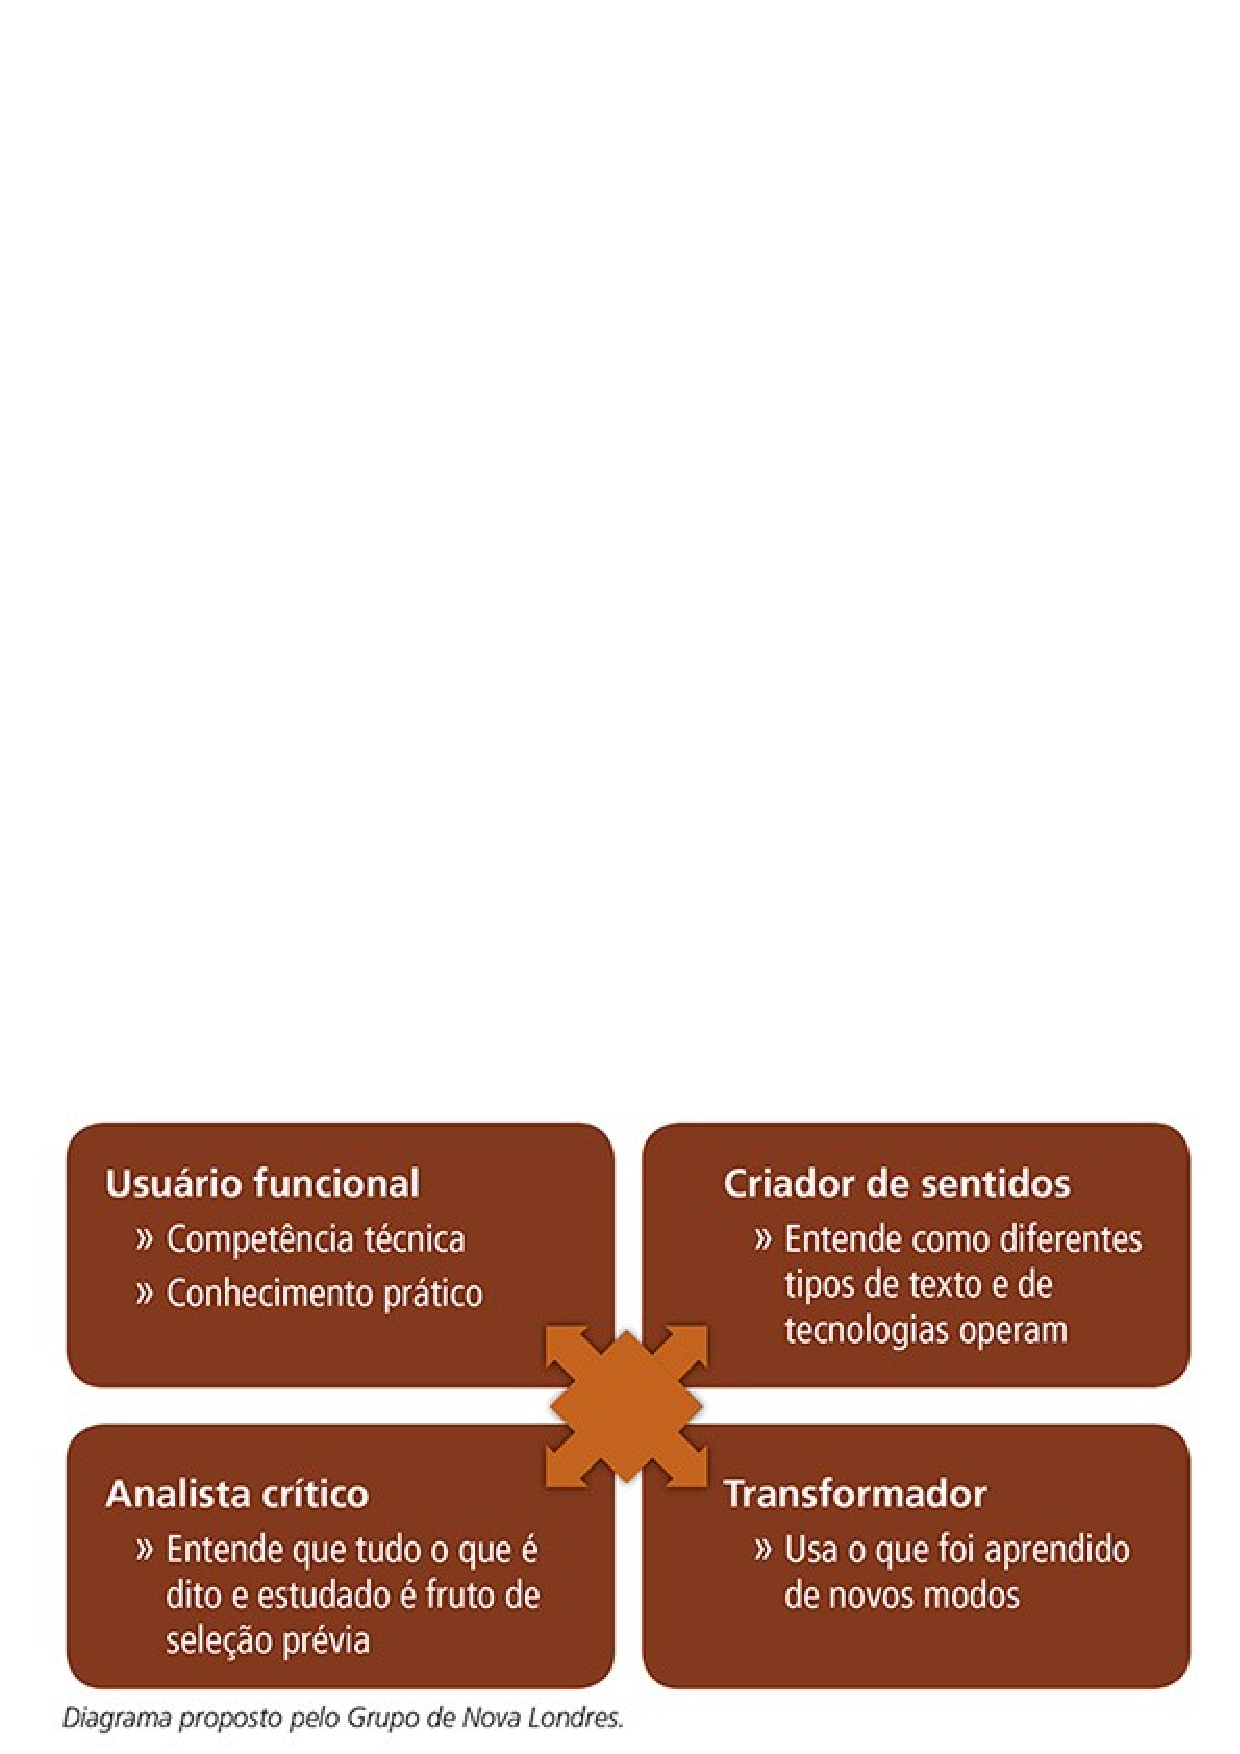
\includegraphics[width=\textwidth]{figure01.pdf}
 \caption{Fases de la investigación.}
 \label{fig01}
 \source{Elaboración propia. Adaptación de \textcite{cambra2033}}
\end{minipage}
\end{figure}


\section{Resultados}
El desarrollo de los resultados se vincula a las fases de la investigación \Cref{fig01} en relación con los diferentes objetivos con una intención secuencial.

\subsection{Fase 1. Descripción de datos}
En esta primera fase se realizó una búsqueda editorial de los diferentes libros de literatura juvenil e infantil que incorporaban epitextos virtuales públicos, en concreto, book-trailer. Esta exploración generó un corpus de 70 libros para los que las editoriales habían alojado en su plataforma virtual algún book-trailer —\Cref{tab03}—.


\begin{table}[h!]
\centering
\begin{threeparttable}
\caption{Epitextos editoriales y destinarios literarios.}
\label{tab03}
\begin{tabular}{l l *{3}{S[table-format=3.0]}}
\toprule
\textbf{Editoriales} & \textbf{Epitextos vituales} & \textbf{Literatura infantil} & \textbf{Literatura juvenil} & \textbf{Total editorial} \\
\midrule
\multirow{3}{*}{Anaya} & Book-trailer (n) & 1 & 8 & 9   \\
& Editorial (\%) & 11,1 & 88,9 & 100  \\
& Corpus (\%) & 2,9 & 22,2 & 12,9 \\
\multirow{3}{*}{Santillana} & Book-trailer (n) & 9 & 0 & 9 \\
& Editorial (\%) & 100,0 & 0,0 & 100 \\
& Corpus (\%) & 26,5 & 0,0 & 12,9 \\
\multirow{3}{*}{SM} & Book-trailer (n) & 16 & 24 & 40 \\
& Editorial (\%) & 40,0 & 60,0 & 100 \\
& Corpus (\%) & 47,1 & 66,7 & 57,1 \\
\multirow{3}{*}{Edelvives} & Book-trailer (n) & 8 & 4 & 12 \\
& Editorial (\%) & 66,7 & 33,3 & 100 \\
& Corpus (\%) & 23,5 & 11,1 & 17,1 \\
\multirow{2}{*}{Total corpus} & Book-trailer (n) & 34 & 36 & 70 \\
& Corpus (\%) & 48,6 & 51,4 & 100 \\
\bottomrule
\end{tabular}
\source{Programa estadístico SPSS.}
\end{threeparttable}
\end{table}


En dicho corpus observamos que, en su conjunto, existe una distribución cercana en el empleo del book-trailer ateniendo a los destinatarios —48,6\%, literatura infantil; y 51,4\%, literatura juvenil—; sin embargo, se convierte en decisión editorial la vinculación de este epitexto a los destinatarios. Es el caso de Santillana que presenta el 100\% o Edelvives (66,7\%) para los primeros lectores, frente a Anaya que tiende a utilizarlo para lectores adolescentes (88,9\%) y SM, en donde hay un mayor equilibrio en su distribución (40\% y 60\%, respectivamente). De lo que podemos obtener una primera aproximación del estudio al considerar que es un recurso empleado en la promoción de la lectura identitaria a lectores infantiles y juveniles, pues se advierte la ausencia de este recurso para las colecciones editoriales destinadas a los autores clásicos, que también forman parte del canon escolar y que su acercamiento constituye un reto educativo \cite{garcia2016odio}.



\subsection{Fase 2. Análisis categórico}

Una vez delimitado el corpus editorial, se procede a realizar el análisis de los diferentes book-trailer, utilizando una parrilla de contenidos elaborada \emph{ad hoc} —\Cref{tbl02}—. Se establecen tres categorías de análisis: características, modalidades y aportaciones didácticas. Así, dentro de la primera categoría, se disponen, como se detallan en la \Cref{tbl02}, tres subcategorías vinculadas a los ítems de las características —paratextos del libro-objeto (ítems 1 a 7), técnicas cinematográficas (ítems 8 a 14) a e interacción con el lector (ítems 15 a 20)—.

\subsection{Fase 3. Análisis interpretativo}

El estudio de las características de los epitextos vituales —\Cref{tbl02}, ítems %\ref{itm1,itm2,itm3,itm4,itm5,itm6,itm7,itm8} 
1 a 8— se ha realizado atendiendo a dos perspectivas: por un lado, en torno a las editoriales en sí mismas —\Cref{fig02}—; y, por otro, en relación con la distribución de los paratextos en relación con los destinatarios, atendiendo a la literatura infantil o juvenil —\Cref{tab04}—. En el caso de los paratextos, destaca la inclusión de la cubierta por parte de las editoriales, sobre todo, al final del book-trailer —ítem 2—, con porcentajes superiores al 90\%, frente a su aparición al inicio —ítem 3—, no llegando a superar el 16,7\% por parte de Edelvives. Son estrategias cuyo objetivo es mantener la intriga del mensaje y resaltar la materialidad del libro para su promoción y consumo \cite{garcia2013papel}. Sin embargo, los metadatos se centran principalmente en la entradilla —ítem 4—, con porcentajes que oscilan entre el 83,3\% y el 55,6\%, ya que quedan poco representados los referidos al punto de venta —ítems 6— o a la fecha de lanzamiento —ítems 7—, que ofrecen resultados residuales, en ocasiones sin presencia. 

Un aspecto relevante, por su relación con la obra en sí, es la presencia de datos relacionados con el autor —ítem 5— y con referencias de algún texto de la obra —ítem 7—. Si bien la información sobre el autor mantiene un porcentaje en torno al 40\% en todas las editoriales; sin embargo, se observa una baja presencia de textos originales de las obras que oscilan entre el 58,3\%, en Edelvives, a un 0\%, en Santillana \cite{lluch2003analisis}. Este aspecto debería cuidarse por parte de las editoriales y no convertir estos productos virtuales en \emph{sustitutos transmedia} de la obra original, ya que podríamos dispersar el objeto prioritario: la formación de lectores. 

\begin{figure}[htbp]
\centering
\begin{minipage}{.8\textwidth}
 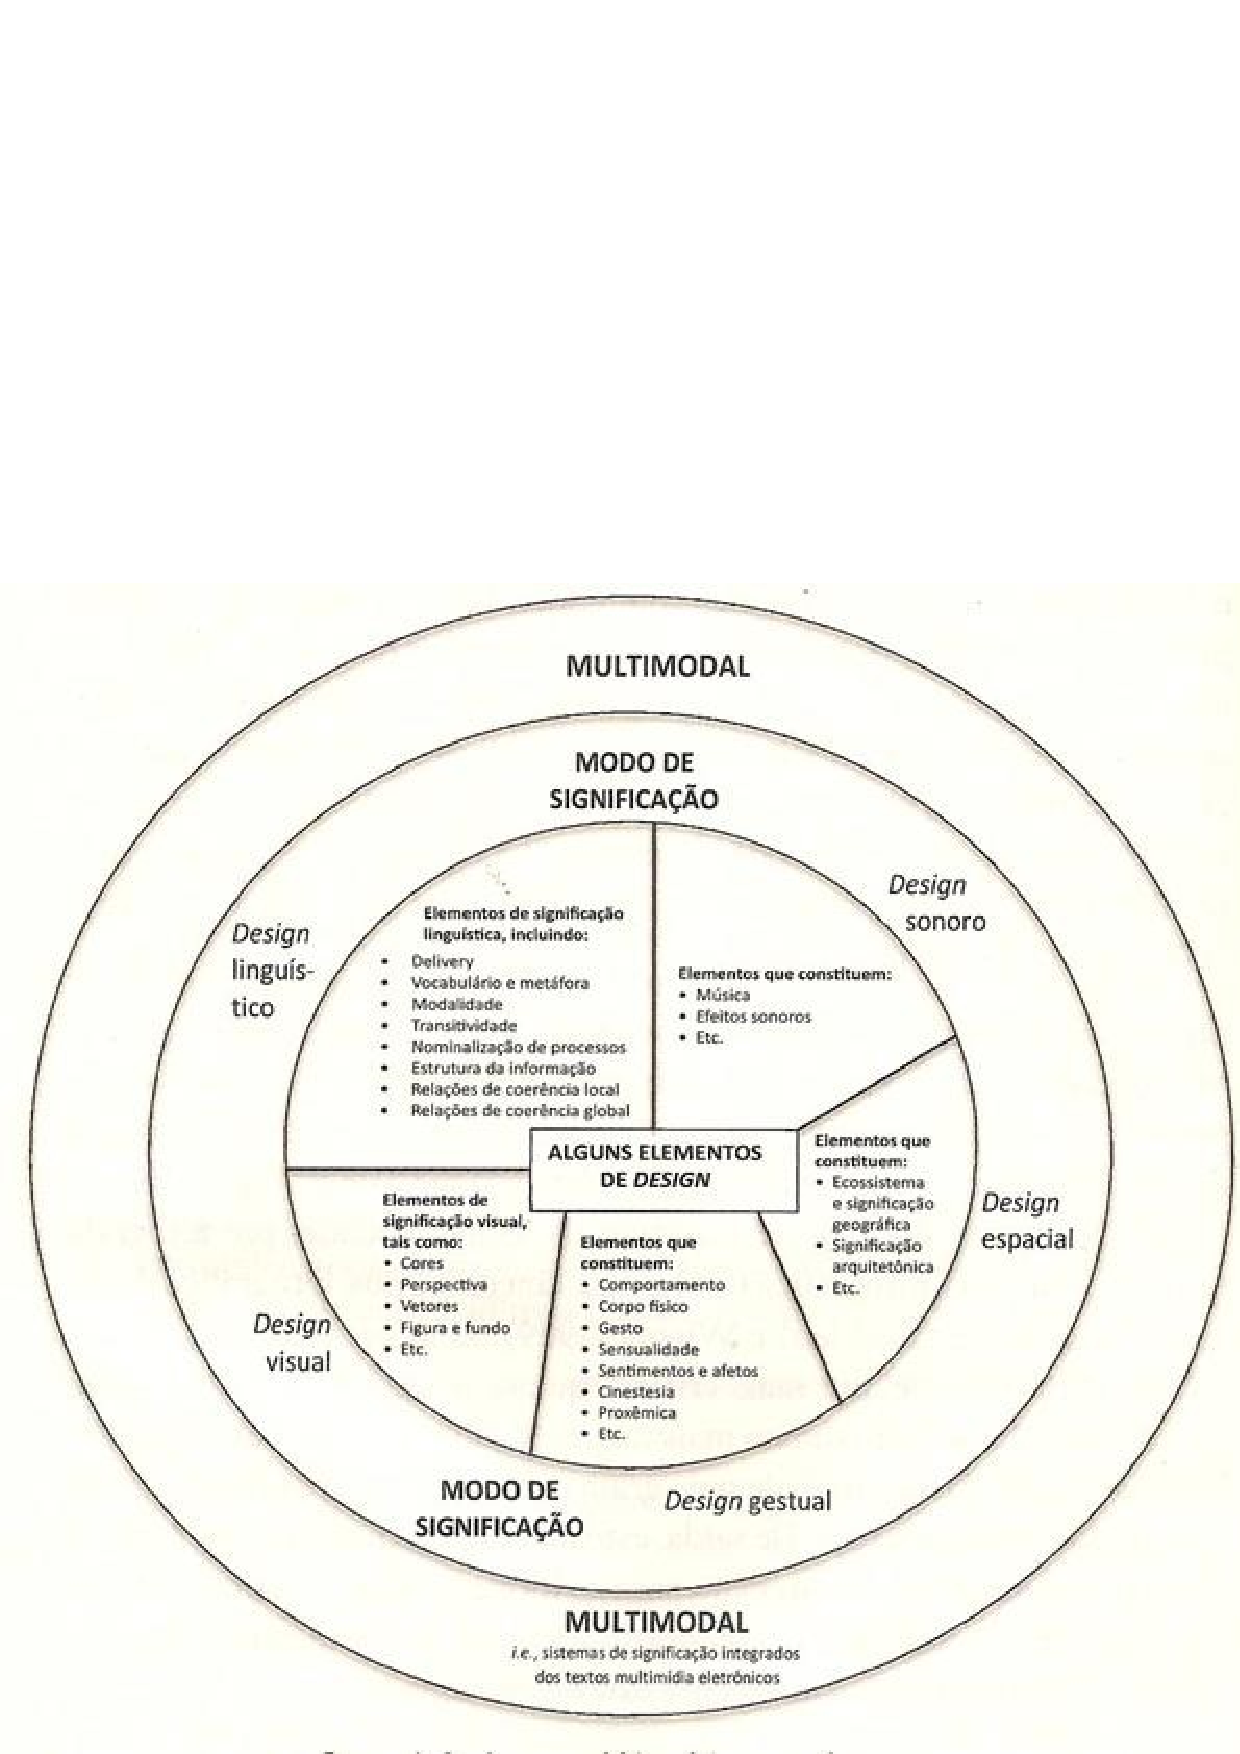
\includegraphics[width=\textwidth]{figure02.png}
 \caption{Distribución de los paratextos en las editoriales.}
 \label{fig02}
 \source{Programa estadístico SPSS.}
\end{minipage}
\end{figure}

Si bien la distribución de características por editoriales ofrece un perfil de la estrategia de promoción de libro \cite{landow2015bueno}, no podemos obviar cómo se distribuyen respecto a los destinatarios lectores —\Cref{tab04}—. Se observa que una tendencia superior de ofrecer metadatos (ítems 1 y 3) que se vinculan a las comunidades lectoras y las sagas de libros y series televisivas \cite{rovira022evolucion}, ya que se convierte en una información interesante para el adolescente y sus iguales. Este dato se une a la información sobre el autor (ítem 5) que también es vinculante a los lectores con mayor formación literaria.  

\begin{table}[h!]
\centering
\begin{threeparttable}
\caption{Distribución de paratextos según los destinatarios.}
\label{tab04}
\begin{tabular}{*{3}{l} *{2}{S[table-format=3.0]}}
\toprule
\textbf{ítem} & \textbf{Características} & \textbf{Resultados} & \textbf{Literatura infantil} & \textbf{Literatura juvenil} \\
\midrule
 \multirow{2}{*}{1} & \multirow{2}{*}{Información sobre fecha de lanzamiento} &(n) & 0 & 5   \\
& & (\%) & 0 & 13,9 \\
 \multirow{2}{*}{2} & \multirow{2}{*}{Cubierta del libro al final} & (n) & 34 & 34 \\
& & (\%) & 100 & 94,4 \\
 \multirow{2}{*}{3} & \multirow{2}{*}{Cubierta del libro al principio} & (n) & 5 & 3 \\
& & (\%) & 14,7 & 8,3 \\
 \multirow{2}{*}{4} & \multirow{2}{*}{Entradilla de presentación y editorial} & (n) & 23 & 27\\
& & (\%) & 67,6 & 75 \\
 \multirow{2}{*}{5} & \multirow{2}{*}{Información sobre el autor} & (n) & 9 & 18 \\
& & (\%) & 26,5 & 50 \\
 \multirow{2}{*}{6} & \multirow{2}{*}{Información sobre punto de venta} & (n) & 1 & 2 \\
& & (\%) & 2,9 & 5,6 \\
 \multirow{2}{*}{7} & \multirow{2}{*}{Textos seleccionados de libro original} & (n) & 14 & 11 \\
& & (\%) & 41,2 & 30,6 \\
\bottomrule
\end{tabular}
\source{Programa estadístico SPSS.}
\end{threeparttable}
\end{table}


Una vez analizado la dimensión de las características y los paratextos del book-trailer, abordamos las técnicas cinematográficas que se emplean en la construcción de estos epitextos virtuales —\Cref{fig03}—. Se observa cómo la brevedad —ítem 8— aparece en todas las editoriales frente al símbolo —ítem 9— y los movimientos de acercamiento —ítem 10—, convirtiéndose Santillana la que presenta mayor representación de estas técnicas. A ella se une un lenguaje audiovisual, caracterizado por tres elementos: la palabra textualizada —ítem 12—, la música —ítem 11— y el zoom —ítem 14—, recursos propiamente cinematográficos que pretenden crear un ambiente y focalizar la información de un mensaje encauzado a crear la curiosidad por la trama y el disfrute del libro \cite{ambros2020cine}. En el lado contrario, el movimiento de acercamiento —ítem 10— es un recurso poco frecuente y ofrece como porcentaje más alto el 22,2\% en Santillana, así como los símbolos —ítem 13— con una representación casi inexistente en las editoriales.

\begin{figure}[htbp]
\centering
\begin{minipage}{.8\textwidth}
 \includegraphics[width=\textwidth]{figura03.png}
 \caption{Relación de las técnicas cinematográficas con las editoriales.}
 \label{fig03}
 \source{Programa estadístico SPSS.}
\end{minipage}
\end{figure}

Si nos centramos en los destinatarios —\Cref{tab05}—, la distribución de los porcentajes es semejante tanto en ambas literaturas. Solamente existe una diferencia destacable en el ítem 9 que solo aparece en los book-trailer de literatura juvenil, aunque con un porcentaje bajo 13,9\% debido a la mayor competencia lectoliteraria del receptor adolescente frente al infantil.

\begin{table}[h!]
\centering
\begin{threeparttable}
\caption{Distribución de técnicas cinematográficas según los destinatarios.}
\label{tab05}
\begin{tabular}{*{3}{l} *{2}{S[table-format=3.0]}}
\toprule
\textbf{ítem} & \textbf{Técnicas cinematográficas} & \textbf{Resultados} & \textbf{Literatura infantil} & \textbf{Literatura juvenil} \\
\midrule
 \multirow{2}{*}{8} & \multirow{2}{*}{Brevedad} & (n) & 34 & 36   \\
& & (\%) & 100 & 100 \\
 \multirow{2}{*}{9} & \multirow{2}{*}{Elipsis} & (n) & 16 & 12 \\
& & (\%) & 47,1 & 33,3 \\
 \multirow{2}{*}{10} & \multirow{2}{*}{Movimientos de acercamiento} & (n) & 5 & 4 \\
& & (\%) & 14,7 & 11,1 \\
 \multirow{2}{*}{11} & \multirow{2}{*}{Música} & (n) & 34 & 30\\
& & (\%) & 100 & 83,3 \\
 \multirow{2}{*}{12} & \multirow{2}{*}{Palabras} & (n) & 29 & 33 \\
& & (\%) & 85,3 & 91,7 \\
 \multirow{2}{*}{13} & \multirow{2}{*}{Símbolos} & (n) & 0 & 5 \\
& & (\%) & 0 & 13,9 \\
 \multirow{2}{*}{14} & \multirow{2}{*}{Zoom} & (n) & 26 & 23 \\
& & (\%) & 76,5 & 63,9 \\
\bottomrule
\end{tabular}
\source{Programa estadístico SPSS.}
\end{threeparttable}
\end{table}

La tercera subdimensión de la caracterización de los book-trailer supone analizar los aspectos referidos a la interacción con el lector —\Cref{fig04}—.

\begin{figure}[htbp]
\centering
\begin{minipage}{.8\textwidth}
 \includegraphics[width=\textwidth]{figura04.png}
 \caption{Distribución de las interacciones con el lector por editorial.}
 \label{fig04}
 \source{Programa estadístico SPSS.}
\end{minipage}
\end{figure}

Se puede apreciar que la característica que mayor presencia tiene es la imagen —ítem 16—, con más de un 50\% en todas, excepto en Santillana que solo un 44,4\%. La distribución de estrategias es homogénea en todas las editoriales que distribuyen en dos bloques las técnicas: por un lado, un porcentaje medio, que oscila entre el 25\% y el 40\%, con el empleo de la voz narrativa —ítem 20—, las preguntas —ítem 18— y la suspensión —ítem 19—, con una clara intención de generar una comunicación hacia la trama, la identidad y la curiosidad del lector. Sin embargo, entre las técnicas sin presencia significativa, está el ítem 15, con ausencia de formas imperativas en dos editoriales para condicionar y mediar al lector.

\begin{table}[h!]
\centering
\begin{threeparttable}
\caption{Relación de las interacciones con el lector con los destinatarios.}
\label{tab06}
\begin{tabular}{*{3}{l} *{2}{S[table-format=3.0]}}
\toprule
\textbf{ítem} & \textbf{Interacción con el lector} & \textbf{Resultados} & \textbf{Literatura infantil} & \textbf{Literatura juvenil} \\
\midrule
 \multirow{2}{*}{15} & \multirow{2}{*}{Formas imperativas} & (n) & 4 & 1   \\
& & (\%) & 12,1 & 3,4 \\
 \multirow{2}{*}{16} & \multirow{2}{*}{Imagen} & (n) & 22 & 17 \\
& & (\%) & 66,7 & 58,6 \\
 \multirow{2}{*}{17} & \multirow{2}{*}{Preguntas} & (n) & 8 & 13 \\
& & (\%) & 24,2 & 44,8 \\
 \multirow{2}{*}{18} & \multirow{2}{*}{Suspensión} & (n) & 7 & 8 \\
& & (\%) & 21,2 & 27,6 \\
 \multirow{2}{*}{19} & \multirow{2}{*}{Voz} & (n) & 11 & 8 \\
& & (\%) & 33,3 & 27,6 \\
\bottomrule
\end{tabular}
\source{Programa estadístico SPSS.}
\end{threeparttable}
\end{table}

La \Cref{tab06} ofrece la posibilidad de comprobar si existen diferentes estrategias para interactuar según el destinatario del book-trailer. Se observa que todas las técnicas presentan porcentajes homogéneos y solo se produce una diferencia significativa en las formas imperativas —ítem 15— que cuatro de las cinco presencias de este recurso se adscriben a la literatura infantil.

La segunda dimensión de estudio se corresponde con la modalidad —\Cref{fig05}—. Las editoriales optan por dos modalidades: cortometrajes de animación —ítem 20— y técnica cinematográfica —ítem 21—, quedando la publicación digital en la modalidad \emph{Issuu} con poca representatividad, en torno al 15\% editorial y sin presencia en Santillana. 

\begin{figure}[htbp]
\centering
\begin{minipage}{.8\textwidth}
 \includegraphics[width=\textwidth]{figura05.png}
 \caption{Relación de las modalidades con las editoriales.}
 \label{fig05}
 \source{Programa estadístico SPSS.}
\end{minipage}
\end{figure}

El cortometraje de animación es utilizado más por SM (67,7\%) y Anaya (66,7\%). En cuando a la segunda, técnica cinematográfica, la utiliza más Santillana con un 55,6\%. Y, por último, \emph{Issuu} aparece más en Edelvives, aunque con un 16,7\% y, en cambio, no lo utiliza ninguno de la editorial Santillana —\Cref{fig05}—.

En cuanto a los destinarios —\Cref{tab07}—, la técnica más usada en ambos es el cortometraje de animación, aunque con una mayor presencia en la literatura infantil (76,5\%). Sobre la técnica cinematográfica, es utilizada más en la literatura juvenil, pero no llega ni al 40\%. Y, por último, \emph{Issuu} tiene muy poca presencia en juvenil (8,3\%), con cierta representación en la literatura infantil, con un 14,7\%.

\begin{table}[h!]
\centering
\begin{threeparttable}
\caption{Distribución de modalidades según destinatarios.}
\label{tab07}
\begin{tabular}{*{3}{l} *{2}{S[table-format=3.0]}}
\toprule
\textbf{ítem} & \textbf{Interacción con el lector} & \textbf{Resultados} & \textbf{Literatura infantil} & \textbf{Literatura juvenil} \\
\midrule
 \multirow{2}{*}{20} & \multirow{2}{*}{De cortometraje de animación} & (n) & 26 & 21   \\
& & (\%) & 76,5 & 58,3 \\
 \multirow{2}{*}{21} & \multirow{2}{*}{De técnica cinematográfica} & (n) & 9 & 13 \\
& & (\%) & 26,5 & 36,1 \\
 \multirow{2}{*}{22} & \multirow{2}{*}{\textit{Issuu}} & (n) & 5 & 3 \\
& & (\%) & 14,7 & 8,3 \\
\bottomrule
\end{tabular}
\source{Programa estadístico SPSS.}
\end{threeparttable}
\end{table}

Finalmente, la última dimensión de estudio —\Cref{tbl02} —se refiere a la finalidad del epitexto virtual. Se observa que ninguna de las editoriales los vincula con una propuesta docente —ítem 24— ni colectiva —ítem 25—. En cambio, la informacional aparece como forma generalizada en todas editoriales y vinculadas a los destinatarios de literatura infantil y juvenil.

\section{Discusión y conclusiones}

El análisis de la promoción de la lectura mediante epitextos virtuales ha evidenciado que las plataformas editoriales educativas han incorporado nuevos lenguajes en consonancia con la sociedad en la que se desarrollan las prácticas letradas de primeros lectores y adolescentes. Se ha realizado un estudio de book-trailer y se ha atendido a la categorización de tres dimensiones que abarcan no solo sus características —\emph{Paratextos del libro-objeto}, \emph{Técnicas cinematográficas}, \emph{Interacción con el lector}—, sino su vinculación con los procesos trasmedia —técnicas de elaboración del epitexto— y las intenciones y funcionalidad hacia la promoción del libro.

Los resultados obtenidos coinciden con otras investigaciones referidas a los book-trailer centradas en los libros informacionales \cite{tabernero2022promocion}, en el desempeño de la formación de profesorado \cite{romero2019book}, en el desarrollo de hábitos lectores en LIJ \cite{rovira2017booktrailer} o en el desarrollo de la competencia comunicativa, literaria y digital \cite{ibarra2016book}. Sin embargo, siendo conscientes de que la lectura obedece a un nuevo paradigma orquestado por un ecosistema social \cite{bronfenbrenner1983,bronfenbrenner_ecologia_1987}, nuestra investigación ha pretendido indagar en los grupos editoriales que, en la actualidad, amplían su labor tradicional y emplean nuevas estrategias desde la concepción del libro-arte \cite{colman2007new} y los procesos transmedia mediante la edición de estos epitextos virtuales, diferenciando las estrategias que predominan para destinatarios de literatura infantil y de literatura juvenil, observándose que emplean las mismas técnicas en ambos casos —\Cref{tab03}—. 

Además, se haya evidenciado que la incorporación de los book-trailer en las plataformas editoriales adquieren la función de mediación y prescripción hacia el lector —ítem 23— y que utilizan estrategias multimodales propias de la animación —ítem 20— y del cine —ítem 21— en donde incorporan diversos elementos partextuales, como la cubierta del libro —ítems 2 y 3—. Una constelación de ideas para que el lector se sienta atraído por este formato ficcional: su brevedad —ítem 8— y las técnicas cinematográficas están al servicio del consumo y la promoción del libro. Así, se constata que este epitexto se integra en el nuevo paradigma de la lectura en el que converge la hibridación de elementos analógicos y digitales \cite{wolf2020,kovac2020lectura} y el papel de los grupos editoriales en la promoción del libro mediante epitextos ficcionales transmedia, materializados en los book-trailer, aprovecha los momentos de una cultura snack \cite{scolari2021} en la que se precisa velar por el propio libro y su lectura. Podemos estar cayendo en la viralidad de las modas en una literatura de hipermercado y ventas. El texto y su lectura es la prioridad en nuestro caso, la promoción es el medio y los epitextos virtuales han de convertirse en la estrategia para acercar el disfrute del hecho literario en esta sociedad en la que prevalece la imagen y el sonido frente a la palabra, dicho de otra manera, la fugacidad frente a lo estático y perdurable. 

Finalmente, se debe indicar que, entre las limitaciones y prospección del estudio, se presenta dar voz a los propios prosumidores de la lectura en esta sociedad gaseosa y ver cómo todas estas estrategias repercuten en sus decisiones y hábitos lectores. Tanto en sus primeras etapas, como los adolescentes no permanecen ajenos a este nuevo escenario ya que se desenvuelven en esta sociedad gaseosa \cite{scolari2021}, pues, en definitiva, como indican \textcite[p. 19-20]{romero_oliva_habitos_2020}:


\begin{quote}
    En él participan no solo cuestiones intrínsecas a estos jóvenes y su propia identidad lectora (gustos, preferencias, formatos, ocio…), sino también agentes extrínsecos, tanto mediadores institucionales (escuela, bibliotecas escolares, administraciones educativas…) como mediadores no institucionales (familias, iguales, librerías, editoriales, medios de comunicación convencionales y alternativos, como YouTube, \emph{booktubers}, \emph{wattapad}, \emph{instagramers}, etc.).
\end{quote}




\printbibliography\label{sec-bib}
% if the text is not in Portuguese, it might be necessary to use the code below instead to print the correct ABNT abbreviations [s.n.], [s.l.]
%\begin{portuguese}
%\printbibliography[title={Bibliography}]
%\end{portuguese}


%full list: conceptualization,datacuration,formalanalysis,funding,investigation,methodology,projadm,resources,software,supervision,validation,visualization,writing,review
\begin{contributors}[sec-contributors]
\authorcontribution{Manuel Francisco Romero Oliva}[conceptualization,investigation,writing]
\authorcontribution{Hugo Heredia Ponce}[conceptualization,investigation,writing]
\authorcontribution{Carmen Romero Claudio}[conceptualization,investigation,writing,review]
\end{contributors}


\end{document}
